%!TEX root = ../report.tex
\section{Pitchfork}


The cheapest way to continue on the stable, non-symmetric branch of the pitchfork is to break the symmetry of the PDE temporarily. This is carried out by adding a non-symmetric forcing term to the equation controlled by a new parameter, continuing in the new parameter for just two small steps, subsequently continuing in $Re$ past the pitchfork bifurcation point, and then restoring symmetry again.

We add this asymmetry at $Re = 16$ and continue in $Re$ until $Re \approx 31.$ At this point it becomes clear we have passed the pitchfork bifurcation, by inspecting the behaviour of $\psi_{max}.$ Hence, we bring back the new parameter to $0.$ Next we continue to $Re = 40$ at which point we obtain the solution as plotted in Figure~\ref{fig:question_e}.

\begin{figure}[h]
    \centering
    \caption{Solutions on the upper branch of the pitchfork}\label{fig:question_e}
    \centerline{
    \begin{subfigure}[b]{0.6\textwidth}
        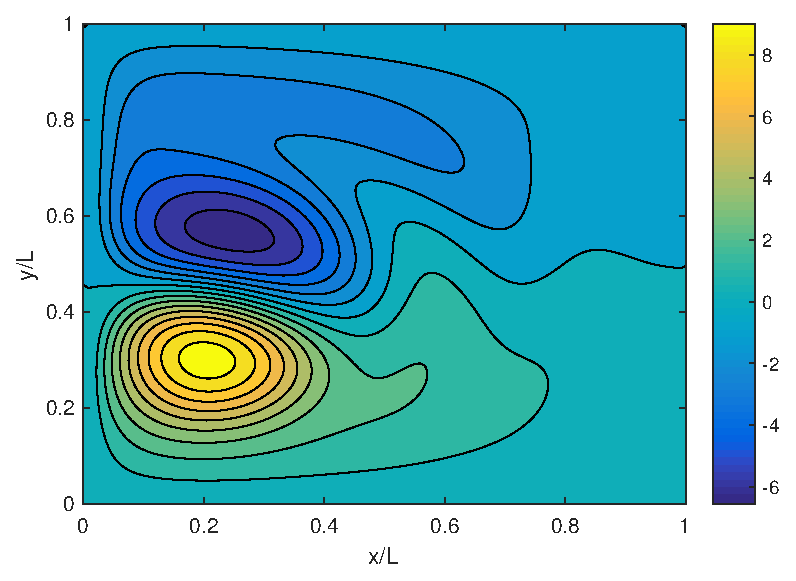
\includegraphics[width=\textwidth]{images/e_psi.eps}
        \caption{Streamfunction $\psi$ at $Re = 40$}
        \label{fig:question_e_psi}
    \end{subfigure}
    ~
    \begin{subfigure}[b]{0.6\textwidth}
        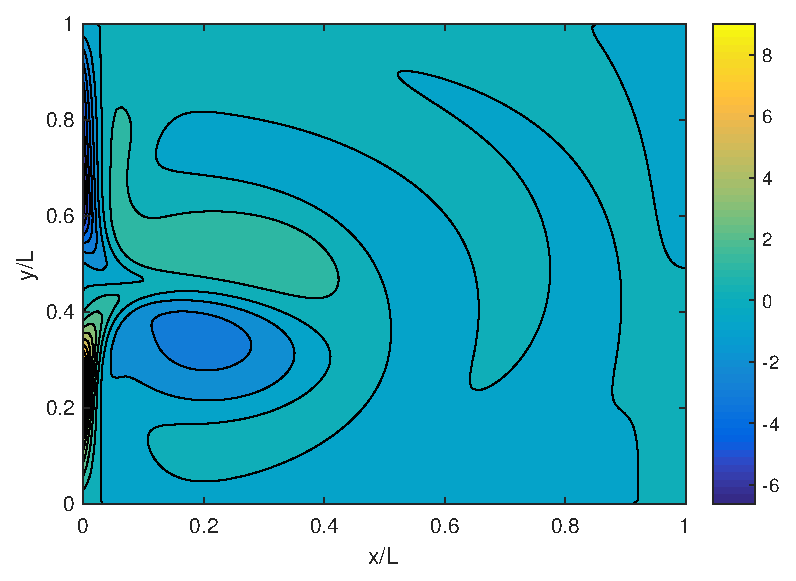
\includegraphics[width=\textwidth]{images/e_zeta.eps}
        \caption{$\zeta$ at $Re = 40$}
        \label{fig:question_e_zeta}
    \end{subfigure}
    }
\end{figure}

Now that we are on asymmetric branch of the pitchfork, we can easily get on its anti-symmetric counterpart by continuing backwards in $Re$ from $Re = 40$ to $Re_p$ and then all the way to $Re = 40$ again. This is done by setting $\Delta s = -1.$ We plot the solution in Figure~\ref{fig:question_e_lower}.


\begin{figure}[h]
    \centering
    \caption{Solutions on the lower branch of the pitchfork}\label{fig:question_e_lower}
    \centerline{
    \begin{subfigure}[b]{0.6\textwidth}
        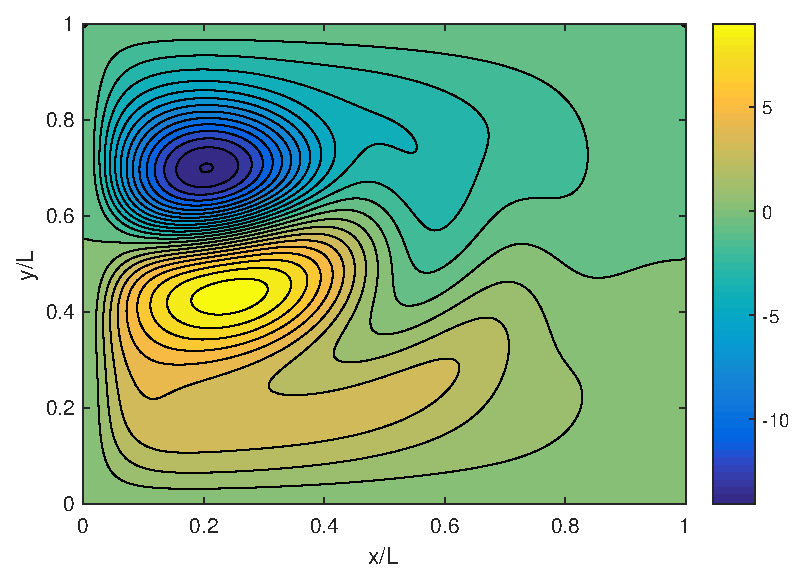
\includegraphics[width=\textwidth]{images/e_psi_lower.eps}
        \caption{Streamfunction $\psi$ at $Re = 40$}
        \label{fig:question_e_psi_lower}
    \end{subfigure}
    ~
    \begin{subfigure}[b]{0.6\textwidth}
        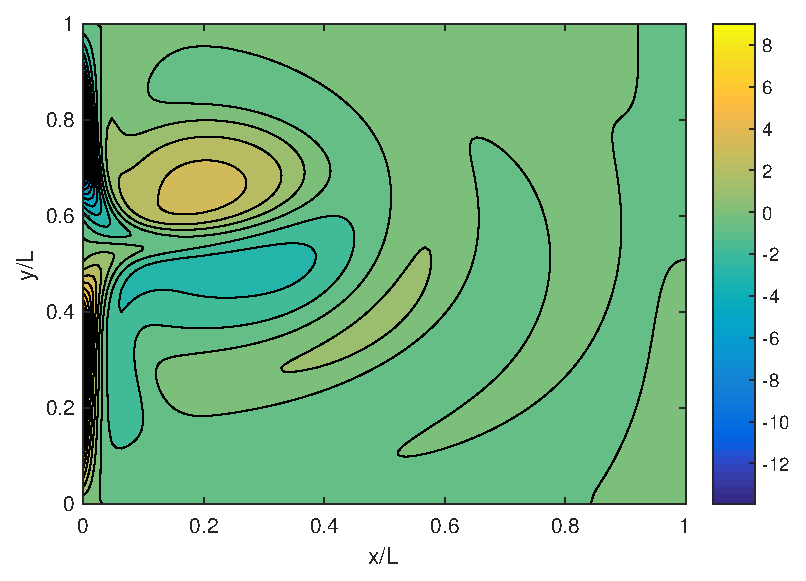
\includegraphics[width=\textwidth]{images/e_zeta_lower.eps}
        \caption{$\zeta$ at $Re = 40$}
        \label{fig:question_e_zeta_lower}
    \end{subfigure}
    }
\end{figure}